\comment{
\begin{figure}
(a) DDMS: show state machine, with databases as states and updates as transitions.

(b) DBMS: database sits and waits for queries to arrive; answers them.

(c) Data stream processor: Set of sitting queries; a stream of data passes by.

\caption{Data management systems architectures: DDMS vs. DBMS vs. data stream processors.}
\end{figure}
}

\begin{figure}
\begin{center}
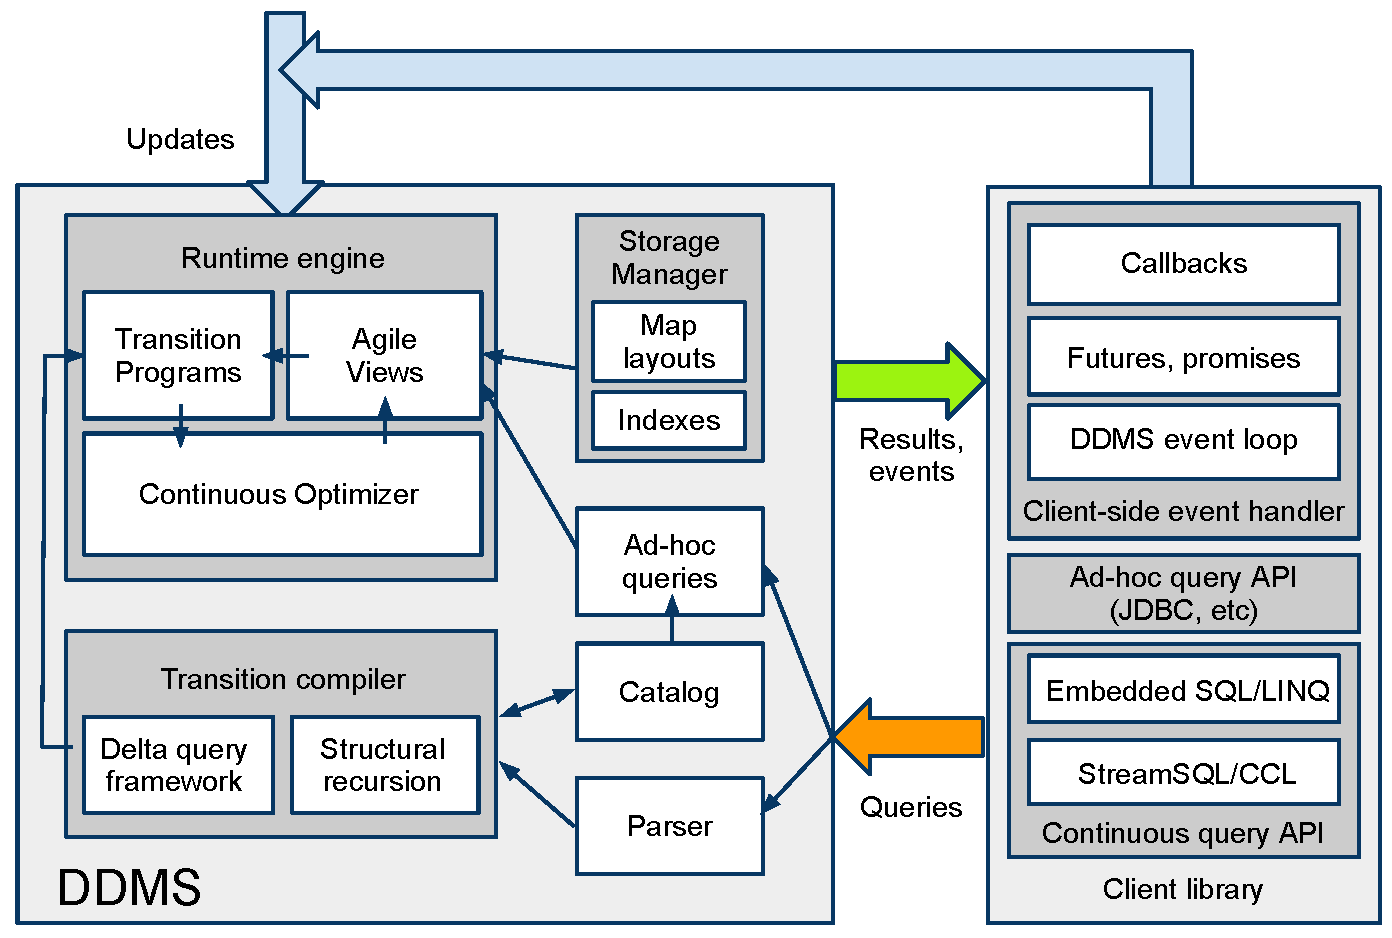
\includegraphics[width=3.3in]{graphics/CIDRarch.pdf}
\end{center}
\vspace*{-0.2in}
\caption{Dynamic Data Management System (DDMS) and Application Interface
Architecture}
\label{fig:ddmsarch}
\vspace*{-0.2in}
\end{figure}

We now examine the architecture of a DDMS, illustrated in Figure \ref{fig:ddmsarch}.  The core component of a DDMS is its runtime engine.  Unlike a traditional database system where the same runtime code manages all database instances, each DDMS runtime is instantiated around a specific set of materialized views that we refer to as its \textit{visible schema}.  The visible schema is the primary read interface between client programs and a DDMS runtime instance.  This interface takes three forms: (1) a read only \textit{dynamic datastructure} representing each view of interest, (2) futures/promises representing queries over the views that have not yet been computed, and finally (3) a push interface that invokes a client callback or schedules an event handler when certain (simple) conditions are met within the visible schema.  If necessary, a DDMS runtime can also be instantiated with support for ad-hoc queries.

Just as we phrase read interface in terms of a traditional DBMS as a set of views, we can phrase the write interface in terms of updates to base relations.  Each DDMS runtime accepts an \textit{update stream} of tuple insertions, deletions and revisions.  The updates are processed, and any changes in the visible schema are propagated to the client.  As an aside, an interesting consequence of this limited visibility is that base relations need not be part of the runtime's state (unless ad-hoc query support is required).  We return to this observation momentarily.

{\bf The runtime state machine}\/.
The internals of the runtime engine itself are best viewed through the lens of a state machine.  Compared to similar abstractions for stream processors\cite{demers-sigmod:07}, the state is substantially larger; conceptually at least, the state represents an entire relational database.  Transitions however, simply represent changes in the base relations: events in the update stream.

{\bf Compiling transitions}\/.
In spite of their apparent simplicity, transitions are quite difficult to evaluate; Each transition is effectively a query for each view of interest.  Though the subqueries are simpler, it is not enough to make a DBMS-style query workload tenable in a high-performance system.  However, instead of reevaluating the subquery on every transition, we can extend the runtime to maintain it as another materialized view.  These views - the \textit{auxiliary schema} - are generated by the DDMS compiler by a recursive decompilation process discussed further in the next section.  

{\bf Space vs speed, partitioning and other optimizations}\/.
The entire \textit{relevant} state of the database can be expressed solely in terms of the auxiliary and visible schemas.  Though the entire relational database need not be stored, there is still substantial overlap between views; the recursive decompilation approach effectively sacrifices space for speed.  Thus, the compiler may drop one or more views in order to keep expected space usage within predefined bounds.  Similarly, the runtime includes a continuous query optimizer that guides the decisions to be made across the database schema, state and storage.  The optimizer's decisions are made in terms of the space being used, the cost of applying transitions on updates, as well as information from a storage manager that aids in physical aspects of handling large states, including implementing a variety of layouts and indexes to facilitate processing.\